\section{Bachelor Angewandte Informatik}
\sidebar{
    \centering
    \includegraphics[width=3cm]{bilder/cant_sleep_1.png}\\\vspace{13mm}
    \includegraphics[width=3cm]{bilder/cant_sleep_2.png}\\\vspace{13mm}
    \includegraphics[width=3cm]{bilder/cant_sleep_3.png}\\\vspace{13mm}
    \includegraphics[width=3cm]{bilder/cant_sleep_4.png}
}

\subsection{Die ersten Semester}

Im ersten Semester hört ihr die Informatikvorlesungen „Einführung in die Praktische Informatik“ und „Einführung in die Technische Informatik“ sowie eine Mathematikvorlesung. Weiterhin ist der „Programmierkurs“ Pflicht, in dem grundlegende Fertigkeiten in C++ vermittelt werden sollen.

In „Einführung in die Praktische Informatik“ (IPI) sollt ihr Programmieren und andere Grundfertigkeiten lernen. Ihr sollt einen Überblick über verschiedene Grundkonzepte der Informatik und Grundkenntnisse in einer oder mehrerer Programmiersprachen bekommen.

Die „Einführung in die Technische Informatik“ (ITE) soll euch Kenntnisse über den grundsätzlichen Aufbau und die Funktionsweise von Rechnern vermitteln. Ihr lernt Schritt für Schritt, angefangen bei Logik und einfachen Schaltungen, wie ein Prozessor und letztendlich ein ganzer Computer funktioniert.


\subsection{\dots{}Später dann}

In den späteren Vorlesungen werden einzelne Themengebiete eröffnet und vertieft, die Namen der Vorlesungen sprechen zum größten Teil für sich, zum Beispiel „Datenbanken“ oder „Betriebssysteme und Netzwerke“.

Außerdem müsst ihr noch ein Proseminar, ein Seminar sowie ein An\-fän\-ger-- und ein Fortgeschrittenen--Praktikum machen. Diese unterscheiden sich von Vorlesungen da von der Modulbeschreibung kein Inhaltliches Thema vorgegeben wird sondern lediglich die Veranstaltungsform.

Im Seminar und Proseminar müsst ihr euch zu einem Thema, das zu Beginn zugeteilt wird, genau informieren und dann einen Vortrag halten in dem ihr den weiteren Seminarteilnehmern das Thema erklärt. Natürlich beschäftigt sich ein Seminar immer mit einem zusammenhängenden Themenbereich. Während bei einem Proseminar theoretisch mehr auf die Art der Präsentation geachtet wird, ist es bei dem Seminar vor allem wichtig einen inhaltlich guten Vortrag zu halten. Diese Trennung ist aber meistens gar nicht so klar.

Bei den Praktika bekommt ihr ein Softwareprojekt das ihr, in einer Gruppe von zwei bis drei Personen, innerhalb eines Semesters schreiben sollt. Dabei habt ihr meist viel Freiheit wie ihr euch die Zeit und die Arbeit einteilt, da ihr lediglich zum Semesterende fertig sein müsst. Das Anfänger-- und Fortgeschrittenen--Praktikum unterscheidet sich in der Regel nur in seiner Komplexität.

\subsection{Mathe und so\dots}

Das Informatikstudium in Heidelberg beinhaltet einen in Vergleich zu anderen Universitäten hohen Anteil an Mathematik. Ihr könnt von Anfang an entscheiden, welche Art der Mathematikausbildung ihr erhalten möchtet. Ihr habt die Wahl zwischen mehreren Varianten.

In der ersten Variante hört ihr die Vorlesungen „Lineare Algebra I“ (im 1. Semester) und „Analysis I“ (im 3. Semester). Alternativ könnt ihr als Ersatz für die „Lineare Algebra I“ und die „Analysis I“ im ersten und zweiten Semester die Veranstaltungen „Mathematik für Informatiker I“ (entspricht etwa „Lineare Algebra I“) und „Mathematik für Informatiker II“ (ersetzt „Analysis I“) hören. Diese Vorlesungen soll den Informatikstudis speziell die Mathematikkenntnisse vermitteln, die sie in ihrem späteren Studium brauchen werden. Diese Veranstaltung bemüht sich solide Mathematikgrundlagen zu vermitteln und versucht einen Bezug zur Informatik herzustellen. Welche Vorlesung ihr hören solltet, wird im \autoref{mafin} diskutiert.

Hinzu kommen noch die Vorlesung „Einführung in die Numerik“ und eins der drei Module „Analysis II“, „Mathematische Logik“ oder „Einführung in die Wahrscheinlichkeitstheorie und Statistik“. Dazu dürft ihr noch bis zu einem Mathematikmodul belegen, das ist aber freiwillig und ihr könntet genauso gut ein Informatikmodul stattdessen belegen,

Die Mathematikmodule unterscheiden sich stark von der Schulmathematik, unterschätzt den Aufwand für die Vorlesungen nicht! Wenn ihr schon wisst, dass ihr euer Informatikstudium mathematisch ausrichten und weitere Mathematikmodule hören wollt und euch vielleicht später sogar im wissenschaftlichen Rechnen spezialisieren möchtet, ist die Variante mit „Linearer Algebra I“ und „Analysis I“ empfehlenswert.

\subsection{Programmieren. Und dann\dots}

\sidebar{
    \centering
    
\includegraphics[width=3cm]{bilder/backing_up_1.png}\\\vspace{5mm}
    
\includegraphics[width=3cm]{bilder/backing_up_2.png}\\\vspace{5mm}
    
\includegraphics[width=3cm]{bilder/backing_up_3.png}\\\vspace{5mm}
    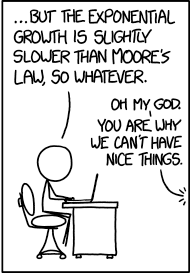
\includegraphics[width=3cm]{bilder/backing_up_4.png}
}

Programmieren ist eine wichtige Fertigkeit. Und die werdet ihr nur teilweise an der Uni lernen. Im „Programmierkurs“ und in der „IPI“ wird versucht, euch die Konzepte näher zu bringen und in den Übungsaufgaben werdet ihr selber kleinere Sachen programmieren müssen.

Es gibt eine enorme Anzahl an Programmiersprachen und die meisten haben ihre Daseinsberechtigung: um praktische Probleme zu lösen, akademisches Interesse oder auch Unterhaltung. Es gibt diverse Paradigmen, nach denen Programmiersprachen konzipiert sind und an der Uni werdet ihr nur die wenigsten kennen lernen. Auch solltet ihr das System kennen, auf dem ihr arbeitet: solide Kenntnisse von unixoiden Systemen, wie Linux und OSX, sind immer Gold wert.

Die Uni hilft aber durchaus: Die „Einführung in die Praktische Informatik“ vermittelt unter anderem grobe Programmierkenntnisse, es gibt den richtigen „Programmierkurs“, der auch Pflicht ist und zur „Einführung in die Numerik“ gibt es praktische Übungen, in denen ebenfalls programmiert wird. Eigeninitiative ist aber dennoch wichtig, mit interessanten Projekten macht das aber auch enorm viel Spaß.


\subsection{Anwendungsgebiet}

Neben dem ganzen Informatik-Kram habt ihr noch ein Anwendungsgebiet. Das ist nicht (wie es sich vielleicht anhört) eine Informatik-Anwendung, sondern einfach ein anderes Fach, in dem ihr einige Veranstaltungen (24 \gls{CP}) hören müsst.

Im Modulhandbuch sind zwar nur einige wenige Fächer als mögliches Anwendungsgebiet aufgelistet, aber das heißt nicht, dass ihr euch nichts anderes anrechnen lassen könnt.

Wenn ihr euch also für andere Fächer mehr interessiert, dann könnt ihr in Absprache mit dem Prüfungsausschuss mit Sicherheit auch dieses Fach hören.

In den meisten Fächern sind die Module, die ihr hören sollt bereits vorgeschrieben. Für gewöhnlich sind dies die Grundmodule des jeweiligen Faches, oft habt ihr jedoch trotzdem einige Wahlmöglichkeiten.


\subsection{Orientierungsprüfung}

Auch in Informatik gibt es eine sog. Orientierungsprüfung. Die besteht darin, dass ihr bis spätestens zum Ende des 3. Semesters die Vorlesung „Einführung in die Praktische Informatik“ bestanden haben müsst.


\subsection{Prüfungen: wie und wieso?}

Zum Thema Prüfungen und Prüfungswiederholungen: Um in den Vorlesungen Creditpoints (meisten mit \gls{CP}) zu bekommen, sprich das Modul abzuschließen, müsst ihr am Ende in den meisten Fällen eine schriftliche Prüfung bestehen. Die genauen Modalitäten, um überhaupt für die Prüfung zugelassen zu werden, legen die DozentInnen jeweils am Anfang des Semesters fest. Informiert euch unbedingt genau, worin die bestehen! Meist müsst ihr am Ende nur im Mittel 50 oder 60 Prozent der Punkte auf den Übungszetteln erreichen, manchmal ist aber auch gefordert, dass jeder Übungszettel bearbeitet wurde.

Ihr solltet euch auch bei jeder Veranstaltung genau darüber informieren, was genau \emph{eine} Prüfung beinhaltet (z.\,B.\ Bestehen von einer von zwei Klausuren). Insbesondere der letzte Teil ist wichtig, denn ihr könnt Prüfungen grundsätzlich zweimal versuchen. Je nach Veranstaltung und Dozent/in \emph{können} zwei Klausuren als eine Prüfung zählen, müssen aber nicht -- dann würde jede geschriebene Klausur als ein Prüfungsversuch gelten. Wenn ihr aus Gründen, die ihr nicht zu verantworten habt (wie krank sein), nicht an einer \emph{Prüfung} teilnehmen konntet, bekommt ihr entsprechend einen Ausweichtermin. Aber keine Panik -- auch wenn ihr in einer Vorlesung zum zweiten Mal die Prüfung nicht bestanden haben solltet, seid ihr noch nicht exmatrikuliert: In bis zu vier Fällen dürft ihr auf Antrag Prüfungen auch ein zweites Mal wiederholen, dies gilt aber nicht für die Orientierungsprüfung und für die Bachelorarbeit.

Denkt dran: Eine Klausuranmeldung ist eine Anmeldung zu einer Prüfung. Wenn ihr euch sicher seid, sie nicht zu bestehen, überlegt euch lieber zweimal, ob ihr euch anmeldet. Das Schöne an eurem Studiengang ist, dass die Noten der Grundpflichtmodule („Einführung in die Praktische Informatik“, „Programmierkurs“, „Einführung in die Technische Informatik“, „Lineare Algebra I“ und „Analysis I“) nicht in eure Abschlussnote zählen, das heißt, dass auch wenn die ersten Semester mit der ganzen Mathematik vielleicht etwas hart sind, eure Abschlussnote darunter nicht unbedingt zu leiden hat.

\marginpar{
	\centering
	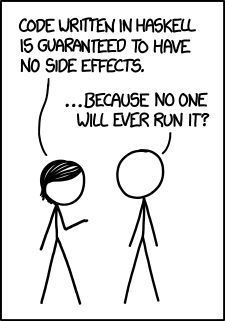
\includegraphics[width=3.5cm]{bilder/haskell.png}
}

\vspace{-\parskip}
